\chapter{Interconnect and Memory Management}
\label{chap:interconnect}

This chapter discusses how the data is transported 
from the main memory to an accelerator and vice versa. 
Essentially, this covers the communication protocol 
and its underlying physical interconnect, 
as well as their impact on system performance 
and software complexity.

The choices made in hardware architecture are 
a trade-off between silicon area, clock speed and flexibility. 
The latter takes the form of restrictions on memory view from the FPGA side, 
which necessitates proper software support 
for the memory allocator and acclerator scheduler.

The software framework, or more precisely, the kernel module
is flexible enough to support a wide diversity of system configurations. 
To demonstrate this, there have been implemented two hardware designs
for the Zynq-7000 series:

The first is geared to accelerator performance featuring
accelerators with deeper pipeline and wider interconnect that allow
greater data processing parallellization.
It has homogenous reconfigurable partitions with
full memory view on the accelerator side, 
allowing a freedom of accelerator placement that
maximizes the scheduler's decision options.

The second one is geared to high accelerator core count 
that sacrifices per-core performance and flexibility.
It uses simpler accelerators with 
narrower and simpler interconnect that lacks buffering.
More importantly, it segments the memory view, 
imposing restrictions on accelerator placement. 
Finally, it features two types of reconfigurable partitions,
further complicating the scheduler.

Furthermore, as part of the effort to port the system
to the newer 64-bit FPGA-SoC from Xilinx, the Zynq UltraScale+,
one more design was created. The accelerator complexity is midway
between the two other designs. Nonetheless, the newer platform's
increased capacity, routing capabilities and 
more flexible partial reconfiguration restrictions
allowed the packing of several times more accelerator instances
operating at much higher frequency.

By providing the correct hardware description 
by the means of a Device Tree\cite{devicetree} data structure, 
the kernel module will be capable to detect and configure the hardware
without the need of source code modification or even a recompilation.

\section{The Communication Protocol}

In order for two (or more) entities to exchange data, 
there must be a well-defined protocol.
With the growth of FPGA ecosystem, a need for a common 
and widespread communication protocol arose
in order to replace custom solutions that deemed 
too inflexible for bigger designs comprising IP
from different project teams and different companies.
The ARM's proposal is the \gls{amba}\cite{amba} protocol suite
which, as the name suggests, was initially deployed 
for microcontroller use but later expanded to SoCs
gaining momentum as a result of ARM's dominance in the smartphone market. 
Since all modern FPGA-SoCs from Xilinx use ARM cores, 
\gls{amba} became a natural choice for the company. 
Earlier products from Xilinx, like Virtex-II Pro which
featured a PowerPC core, used IBM's CoreConnect bus architecture. 
The other big contender is the free and open source ``Wishbone Protocol'', 
which, not unexpectedly, is the favorite of 
``OpenCores'' open-source hardware community.

The Zynq 7000 and the newer Zynq UltraScale+, 
the two platforms that are targeted by this work,
both feature ARM cores and are designed around the \gls{axi} protocol,
part of the \gls{amba} suite. 
As Xilinx tries to promote IP reuse with its IP Integrator tool,
it has expanded the use of \gls{axi} in its FPGAs that contain no ARM IP. 
The \gls{axi} infrastructure and several basic \gls{axi} peripherals
are offered by Xilinx in Vivado at no additional cost.
Therefore, \gls{axi} was chosen for the development of this system.

It is important to note that \gls{amba} protocols are for on-chip interconnect only.
Although they can transverse the PS-PL border,
they are never exposed outside of the chip. 
This stands true not only for Xilinx's -- or Altera's -- FPGAs, 
but also for all ARM-based microcontrollers and SoCs.

\subsection{The AMBA AXI Family}

\label{amba}
The \gls{axi} itself is essentially a group of protocols that support different topologies,
as well as feature levels that position themselves differently at the trade-off 
between performance and functionality versus silicon area.
However, they all share a fundamental bus concept: 
a multi-channel non shared-bus architecture that contains seperate
channels for each \gls{transaction} type. It can be considered as a complementary
to \gls{ahb} protocol, also member of \gls{amba} suite, 
which is a single-channel multiple-master shared-bus architecture. 
Compairing these two families would give an edge to \gls{axi} in
throughtput performance and clock frequency requirements, while \gls{ahb} would favor
better in terms of latency, wire count and power requirements. 
\emph{TODO: να βρω αξιόπιστη πηγή}

Tha \gls{axi} family has several members, but for this system the following three were used:
\begin{itemize}
\item	\textbf{\gls{axi}}, was the initial and only member in \gls{amba} 3.0. 
	With the advent of \gls{amba} 4.0 which introduced
	two new members described below, it is now usually 
	referred as ``Full \gls{axi}'' or ``\gls{axi} Memory Mapped''.
	The characterization of ``full'' contrasts to 
	the reduced capability \gls{axilite} and ``memory mapped''
	contrasts to \gls{axistream} which has no notion of address spaces.

	The \gls{axi} comprises five channels: Read Data (R), Read Address (AR),
	Write Data (W), Write Address (AW), Write Response (B). An \gls{axi} link
	however, may be unidirectional, discarding the unneeded channels.

	Its typical use in the FPGA realm is transferring data between memory resources,
 	like \glspl{bram}, processor RAM, FPGA memory controllers, etc.

	The addressing information must be communicated before a transfer to take place, 
	which consists a performance barrier. 
	To amend this, \gls{axi} supports \gls{burst} mode, 
	where sequential \glspl{beat} of data may be transferred without 
	re-transmitting any addressing information.
	
	\gls{axi} typically needs glue logic 
	between the two endpoints, called ``\gls{axi} Interconnect''. 

\item	\textbf{\gls{axilite}}. Introduced with \gls{amba} 4.0, 
	the \gls{axilite}, as the  name implies,
	is a reduced capability version of \gls{axi}. 
	The most notable simplification is the 
	lack of support for \gls{burst} transfers. 
	In exchange, it offers a much lower silicon footprint. 
	It is best suited for low intensity traffic, 
	typically for configuration or status registers.

\item	\textbf{\gls{axistream}}. Also introduced with \gls{amba} 4.0, 
	\gls{axi}-Stream is a data streaming protocol,
	which means that it has no notion of memory addressing.
	This greatly simplifies implementation and reduces wire count.
	Data flows from the one endpoint to the other, in one direction, 
	without the need of any intermediary interconnect.
	It allows the addition of user defined out-of-band data,
	typically for synchronization, and it supports sender and receiver IDs, 
	which enables stream routing for virtual circuits.
\end{itemize}

None of these protocols supports cache coherency. 
In \gls{amba} 3.0, ARM proposed the \gls{acp}, 
an \gls{axi} slave port that connects an \gls{axi} master directly to the processor.
The coherency logic inside the processor 
will monitor the transactions and update its caches accordingly.
However, since the \gls{axi} master is not aware of the cache coherency logic, 
\gls{acp} is only an \gls{IO Coherency} mechanism;
the processor caches may be coherent but the accelerator's are not.

In \gls{amba} 4.0, ARM extended the \gls{axi} protocol with \gls{ace}, 
which allows full coherency between the processor and the accelerator, 
and \gls{acelite}, an \glslink{IO Coherency}{IO Coherent} version.
The latter differs from \gls{acp} in that its coherency is managed
by the interconnect and therefore the port requires no proximity
to the processor. 
These protocols are supported in the newer UltraScale+ but not in the Zynq-7000.

Finally, in latest \gls{amba} version, 5.0, ARM added \gls{chi}, 
which targets the multiprocessor's local interconnect hub.

In the data streaming model that this work targets, 
there exists no spatial or temporal locality. 
Cached transfers are not only useless but harmful, 
since they will cause cache thrashing. 

Indeed, the kernel driver uses the Linux DMA Streaming API
which bypasses all processor caches by marking 
the allocated DMA'able pages as non-cacheable.
Therefore, cache coherency will not matter our discussion any further;
however, the hardware interconnect that implements these cache-coherent
protocols may be of our use and therefore it will be examined.

\subsection{The AXI Implementation}

The \gls{axi} implementation in Xilinx products consists of the hardware 
implementation in Zynq 7000 and Zynq UltraScale+ devices,
the \gls{soft-ip} protocol infrastructure offered in IP Integrator, 
and the \gls{axi} compatible IP building blocks. 
Additionally, Xilinx offers automation for creating 
custom cores with \gls{axi} interfaces.
It is worth to cover this functionality as 
part of understanding the connectivity of the system.

\subsubsection{The Zynq Hard IP}

The Zynq 7000 is built around \gls{amba} 3.0. 
The interconnect will be presented at the next section,
but it is important to mention here that 
the use of \gls{axi} of this \gls{amba} version
carries two important restrictions: 
The original specification of \gls{axi},
as is present in \gls{amba} 3.0 has a maximum \gls{burst} size of 16. 
Any \gls{axi} master residing in PL that connects to the PS through a slave port,
will have to obey this limit or use a protocol converter.
Secondly, \gls{amba} 3.0 does not support \gls{axilite} or \gls{axistream}, 
therefore all ports in Zynq-7000 are Full \gls{axi}.

The Zynq UltraScale+ is \gls{amba} 4.0 compliant. 
Therefore, both of the aforementioned issues do not apply.
Still, the \gls{afi} that supports the \glsdisp{hp}{HP} ports is version 3 only,
and protocol conversion takes place in silicon. 
This process in transparent to the designer but is still important
as it affects performance.

\subsubsection{The Xilinx Soft IP}
\label{sect:xilinx-ip}

At the PL front, Xilinx offers a suite of 
IP cores that manipulate the \gls{axi} traffic.
It offers cores for conversion (stream combining, 
width conversion), buffering (clock conversion,
stream pipelining, \gls{fifo} buffers) and routing 
(stream broadcasting, stream switching, \gls{axi} crossbar).
Additionally there are some higher level \gls{axi} building blocks
that automate the interconnect of \gls{axi} endpoints. 
Due to their importance, it is worth to be mentioned separately:

\begin{itemize}
\item	\textbf{AXI Interconnect}.
	It can connect $M$ \gls{axi} masters to \gls{axi} $N$ slaves 
	communicating with either the Full \gls{axi},
	both version 3.0 and 4.0, or the \gls{axilite} protocol.
	The interconnect can be configured in full crossbar mode 
	(shared address, multiple data) for high performance,
	or in shared access mode (shared address, shared data) 
	for low area use, issuing only one transaction at a time.
	
	The AXI Interconnect is build around the AXI Crossbar. 
	The AXI Crossbar implements the core switching functionality 
	and the AXI Interconnect wraps it with the appropriate port couplers that may
	perform necessary clock and width conversion and/or append register slices or FIFO buffers,
	to help timing closure and smooth traffic, respectively.

	The AXI Crossbar allows the definition of a connectivity matrix 
	for sparce crossbar implementation. 
	However this feature is not used by AXI Interconnect and if desired,
	the designer must instantiate the AXI Crossbar and its couplers manually.

\item	\textbf{AXI SmartConnect}. 
	This core is a newer design with functionality analogous to \gls{axi} Interconnect.
	It is advertised to be highly optimized to mitigate wire delays in UltraScale+.
	However that comes at some cost in FPGA resources.
	If the design uses a slow clock for the targeted FPGA or 
	if the slaves are \gls{axilite} configuration registers,
	the older \gls{axi} Interconnect should be preferred.

\item	\textbf{AXI Stream Interconnect}. 
	The equivalent interconnect for \gls{axistream}, 
	as it can interface $M$ \gls{axi}-Stream masters to $N$ slaves.
	Likewise its sibling, it is built around the AXI-Stream Switch with the appropriate
	couplers in each of its interfaces.

	The stream routing may either be defined externally through 
	a configuration register or by sender / receiver IDs. 
	It should be stressed that in contrast to its Full \gls{axi} counterparts, 
	it is not an essential core if only a single master is connected to a single slave.
	Its use arises on shared physical links and/or where virtual circuit switching is needed.
\end{itemize}

Xilinx offers a few DMA controllers, compatible with both the full AXI and the AXI Stream.
If implemented in the programmable logic, they can move data between an
addressable memory resource and either another one, or alternatively stream it
to a memoryless component. These are the solutions offered:

\begin{itemize}

\item	\textbf{AXI DataMover}:
	This is the central component of all DMA controllers.
	Its role is to move data between the memory mapped and the streaming domain.
	It needs external logic for control, a role that is assumed
	by the three DMA controllers described below.
\item	\textbf{AXI DMA}:
	The AXI DMA can generate \gls{axistream} compatible streams
	from a full \gls{axi} compatible addressable memory resource.
	Its core are two unidirectional or a single bidirectional
	\footnote{This configuration is not supported by Xilinx HSI for DeviceTree generation,
	which is the standard method describing hardware to the Linux kernel}
	AXI DataMover.
	It is configured by an \gls{axilite} interface.
	The core has an optional scatter-gather engine that can continuously fetch and execute
	transfer descriptors without any pause as well as optional multichannel support.

\item	\textbf{AXI Video DMA}: 
	This core is a variation of the AXI DMA specialized in video streams.
	Among other optimizations, it takes advantage of the user-defined out-of-band channel
	of \gls{axistream} for frame synchronization.

\item	\textbf{Central DMA}: 
	The Central DMA, probably a misnomer, can move data between two Full \gls{axi}
	compatible slaves, e.g. the processor memory and an \gls{axi} BRAM controller.
	It is implemented by a bidirectional DataMover and the control logic, with an optional
	scatter-gather engine. 
 \end{itemize}


\subsubsection{The User IP}

As it becomes clear, Xilinx does offer a significant amount of 
\gls{axi} infrastructure IP and \gls{axi} compatible peripherals
to support the implementation of an \gls{axi}-based system.
Still, implementation of \gls{axi} compliant custom logic is a non-trivial task to undertake.
Depending on the workflow and the designer's experience and demands,
there are five options available.

\begin{itemize}
\item	\textbf{Custom Implementation}:
	In case that maximum flexibility and performance is desired,
	a custom implementation is the way to go. 
	Xilinx offers an \gls{axi} Verification IP 
	which helps the designer to verify the functionality of an RTL design.

\item	\textbf{IP Integrator}:
	Xilinx offers a ``Create and Package IP'' wizard in its IP Integrator tool.
	The designer may define the desired \gls{axi} parameters 
	and the wizard will generate the corresponding RTL code
	to create the \gls{axi} interface. 
	The designer can afterwards tweak the code to adapt their needs.

\item	\textbf{IP Interfaces (IPIFs)}:
	IPIFs are IP cores that alleviate the burden of \gls{axi} conformance 
	from the end designer by performing the complex \gls{axi} signaling 
	themselves while offering a simple memory-like interface on the other end. 
	Xilinx provides two such cores, one for Full \gls{axi} 
	supporting \gls{burst} transactions, and one for \gls{axilite}.

\item	\textbf{Bridges}: In case the user IP is already developed with an alternative protocol,
	it may be possible to be bridged to the \gls{axi} interconnect, 
	if the additional overhead can be tolerated.
	Xilinx provides only a handful of birdges, mostly of use within the \gls{amba} family, 
	e.g. for \gls{ahblite} (both slaves and masters) and for \gls{apb} (slaves only). 
	However, additional bridges may be found at OpenCores or in other open-source libraries. 
	In the simplest case possible, a designer may even opt for 
	the \gls{axi} \gls{gpio} core that can provide up to two 32 bit general purpose I/O lines.

\item	\textbf{HLS}: If the designer uses the Vivado High-Level Synthesis workflow,
	the tool is able generate \gls{axi} compliant IP using simple HLS directives. 
	This is particularily useful to implement the HLS-core control protocol over \gls{axilite}.
\end{itemize}

\section{The Physical Interconnect}

So far, we discussed the communication protocol and its implementation at both 
the programmable logic and the silicon domains.
The next logical step would be to examine the underlying physical interconnect
that supports it on the SoC-FPGAs that this work targets. 

Granted, in the FPGA fabric there is infinite flexibility and any topology may be created.
The presence of a hard IP however, presents a constraining factor.
In both Zynq 7000 and UltraScale+ series, 
there is a single multi-port memory controller
that resides on the PS side. Therefore, any traffic from/to the PL must
first cross the PL-PS boundary, then be routed inside the PS interconnect,
and finally reach a memory controller port. 

Understanding the nature of this path is not a trivial matter. 
Nonetheless, it imposes a number of hardware and software decisions
in this work's implementation, and therefore it needs to be analyzed.

Since the architectural details of these two SoC-FPGA families are
significantly different, they will be covered separately.

\subsection{The Zynq 7000 Interconnect Architecture}

The 7000 series glues the PL and PS together with a number of
high speed ports of varying functionality. Most are slave ports to the
PL, which means the transaction initiator must reside in the programmable logic.
A couple of them are master ports, to be driven by either the ARM cores,
the PS DMA controller or some I/O peripheral. 
One of them is able to provide \gls{IO Coherency},
but there is no support for two-way, full coherency.

The figure \ref{fig:zynq7000-interconnect} presents the system architecture 
of Zynq 7000 series, emphasizing the interconnect. 
Technical details are sourced from \cite{ug585}.

\begin{figure}[htbp]
  \centering
  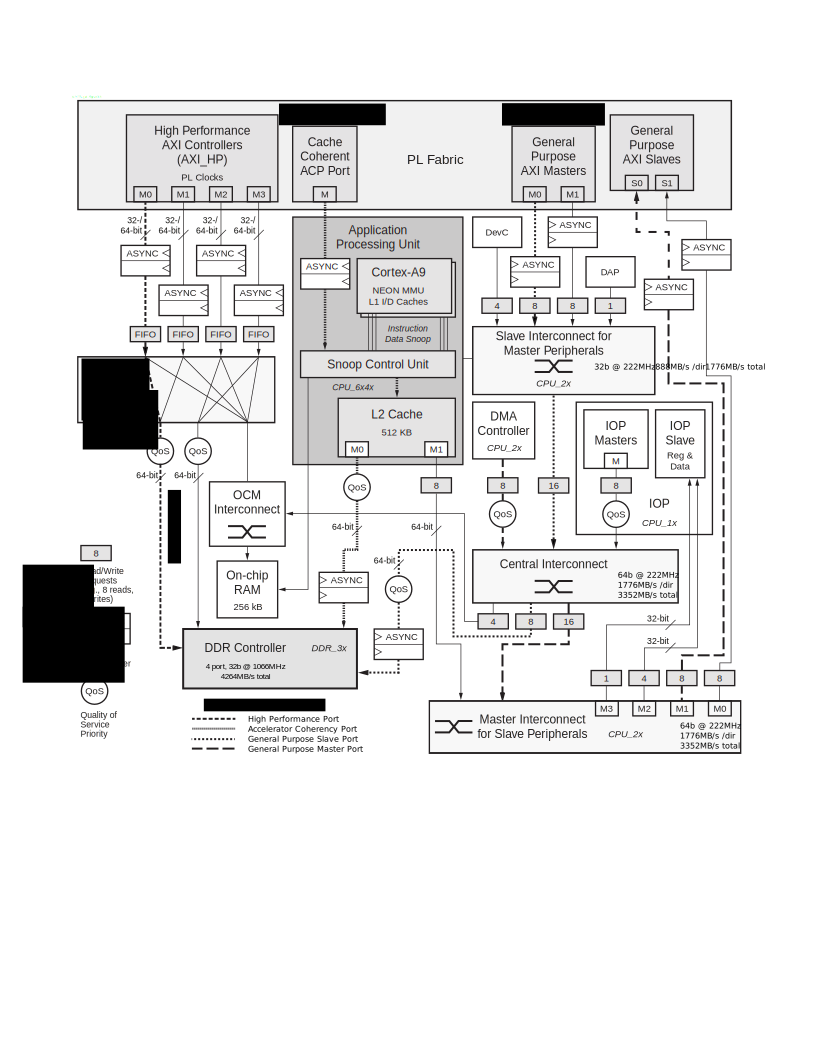
\includegraphics[scale=.9,center,trim={0 75mm 0 0},clip]{img/zynq-7000.pdf}
  \caption{The Zynq 7000 system architecture. 
  Note that port naming follows the controller role, not the port's.
  For example, the ``GP \gls{axi} Masters'' are connected to the
  ``GP \gls{axi} Slave Ports'', titled ``M0'' and ``M1''. Conversely,
  the ``GP \gls{axi} Slaves'' are connected to the ``GP \gls{axi} Master Ports'', titled ``S0'' and ``S1''.
  Modified image from \cite{ug585}.
  }
  \label{fig:zynq7000-interconnect}
\end{figure}

\subsubsection{The High Performance Ports}
\label{sect:zynq7000-hp}

The Zynq 7000 provides four \gls{hp} ports, HP0 to HP3.
These are all slave ports to the PL, conforming to \gls{axi} version 3.
If the \gls{axi} master is implemented in \gls{axi}4, as is the usual case,
protocol conversion must take place in the PL.

The ports are clocked by a PL clock at up to 150MHz, and can be 32 or 64 bit wide.
As the \gls{axi} protocol mandates, they have separate wires for each direction,
offering a per direction bandwidth of 1200MB/s for each port.

The \gls{hp} ports are connected to the memory controller through the Memory Interconnect
which in turn drives two of the four ports of the memory controllers, as well as
one port of the \gls{ocm} interconnect.
The port clock will be converted to 355MHz,
offering a switching speed of 2840MB/s per direction, 5680MB/s total.
The switching scheme routes the traffic from the first two \gls{hp} ports 
to the first memory port, and the other two \gls{hp} ports to the second. 
Any port can be routed to the \gls{ocm}.

The memory controller offers an aggregate bandwidth of 4264MB/s 
shared among its four ports, irrespectively of the data flow direction.
Therefore, if all \gls{hp} ports are used and configured at their maximum ratings,
the maximum theoretical bandwidth of 9600MB/s will saturate the
memory interconnect, and if the OCM path is not used, will be further constricted
by the memory controller.

\subsubsection{The Accelerator Coherency Port}

The \gls{acp} port, compared to the \gls{hp} ports, 
has equivalent performance specifications.
The connectivity to the memory subsystem, 
however, is totally different.
As it was mentioned in \ref{amba}, 
the ACP port needs to be in close proximity to the
processor in order to provide cache coherency 
to traffic generated from a non-coherent \gls{axi} master.
Indeed, in Zynq-7000 series the \gls{acp} port is connected 
directly to the \gls{scu} of the L2 Cache. 
From there, it can access one dedicated 
port of the memory controller.
This is a low latency path to memory, 
but its tight relationship with the processor
will complicate the potential usage scenarios.

\subsubsection{The General Purpose Slave Ports}
\label{sect:sgp}

The GP slave ports offer the half of the data width 
of the \gls{hp} ports as they are 32 bit only,
but they can operate at up to the same frequency of 150MHz. 
However, in order to reach the memory controller 
they follow a much more complicated path.

Firstly they reach the Slave Interconnect. 
They occupy two of its four slave ports,
the other being dedicated to the 
\gls{devc} and the \gls{dap}.
Note that the former will be heavily used at runtime as it is responsible
for programming the FPGA during partial reconfiguration.
The Slave Interconnect operates at 222MHz, 
offering an aggregate bandwidth of 888MB/s per direction.
Its master port is connected to the Central Interconnect, 
which operates also at 222MHz but has a width of 64 bits, 
totalling at 1776MB/s per direction.

The Central Interconnect is shared by another two masters:
The PS DMA controller and the I/O Peripherals
(the flash memory interfaces, the USB and Ethernet controllers, etc).
Itself is a master to three peripherals:
The OCM interconnect to leads to \gls{ocm} memory, the Master Interconnect
which connects the PS masters to the \gls{fabric} via the \gls{mgp} ports,
and finally, one port of the memory controller.

It is obvious that in order for \gls{sgp} to reach the memory controller,
it has to cross two rather busy interconnects and resource competing
could become an issue.

\subsubsection{The General Purpose Master Ports}

The GP master ports are the funcional opposite of GP slave ports;
they can connect PL slaves and they route the traffic through the
Master Interconnect which in turn is a slave to the Central Interconnect.
It is important to note that they are the only master ports from the PS side.
If any transaction has to be started with the initiative of the PS,
it \emph{must} pass from these ports.

\subsection{The Zynq UltraScale+ Interconnect Architecture}

The UltraScale+ series has significantly improved the system interconnect.
Apart from the expected increase in number and bandwidth of the
PS-PL ports and their pathway to the memory, there is much better support
for cache-coherent peripherals. 
Unlike the 7000 series, in UltraScale+ 
all ports are of equal maximum width and frequency; 
they are all 128 bit wide and may operate at up to 333MHz.
Nonetheless, since they have different connectivity and offer different
functionality, subsequently they will also differ in access latency to
the memory controller as well as produce distinct side effects. 
Additionally, they are mapped differently in the
processor address space and have varying address widths; all of them
however, are at least 32 bits.
The UltraScale+ is updated to \gls{axi}4, with the exception of the \gls{afi}.

An overview focused on interconnect
is displayed in figure \ref{fig:zynqmp-interconnect}. 
The reference for technical information presented here is \cite{ug1085}.

\begin{figure}[htbp]
  \centering
  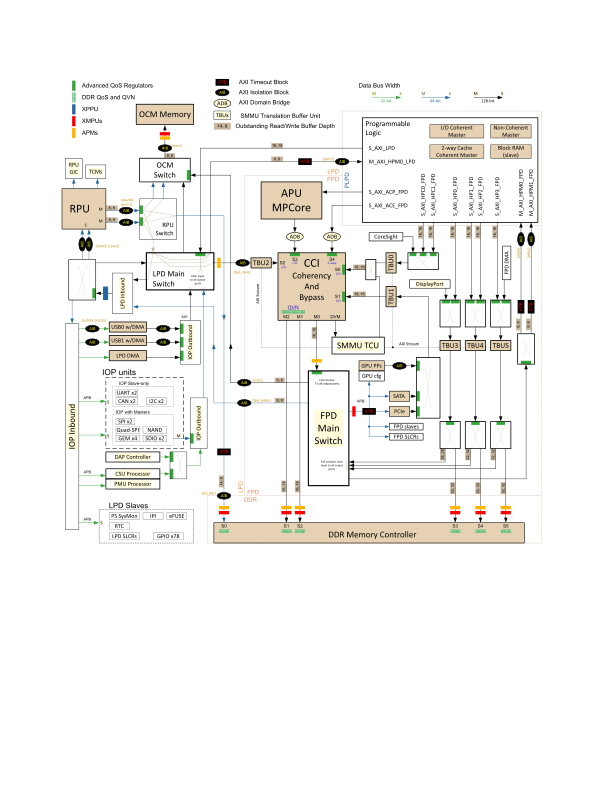
\includegraphics[scale=.9,center,trim={0 75mm 0 0},clip]{img/zynqmp.pdf}
  \caption{The Zynq UltraScale+ system architecture, image from Xilinx \cite{ug1085}.
  The naming nomenclature denotes (in order) the master or slave role, 
  the protocol (AXI), the port name with the modifier ``C'' for ``coherent'' or
  repeating ``M'' for ``master'' then followed by the port number, and finally
  the power domain designation.
  }
  \label{fig:zynqmp-interconnect}
\end{figure}


\subsubsection{High Performance Ports}
\label{sect:implementation}

The UltraScale+ features four \gls{hp} ports that reside in the \glsentrylong{fpd}.
As one can realize from figure \ref{fig:zynqmp-interconnect},
the path from an \gls{hp} port to the memory controller is not identical for all ports.
Indeed, the memory port S3 is shared between the HP0 and the DisplayPort controller
while the S5 is shared between HP3 and the \gls{fpd} DMA.
The interfaces HP1 and HP2 share exclusive access to memory port S4,
a property to be considered if the lowest latency 
or a deterministic performance is desired. Additionally, if the DisplayPort
controller is not used, the HP0 will have full bandwidth access to the S3 memory port.
The HP3 would be the least attractive to use, 
since the memory access pattern of the \gls{fpd}
DMA may not always be known in advance.

\subsubsection{High Performance Coherent Ports}

As the name suggests, the \gls{hpc} ports are cache-coherent versions of \gls{hp}, 
albeit \glslink{IO Coherency}{IO coherent} only, much like the \gls{acp} port. 
However, in contrast to the \gls{acp},
the coherency is not ensured by the \gls{scu} but by the \gls{cci}.

Decoupling the port from the processor has both its benefits and its shortcomings. 
The \gls{hpc} ports have higher latency than \gls{acp} to the memory controller,
even higher than \gls{hp} ports since they have to cross \gls{cci}.
On the other hand, it does not share a path with the processor to the cache,
alleviating the resource competing in a such an important pathway.
Xilinx labels the \gls{acp} as a ``legacy'' port, 
showing its preference in \gls{hpc}.

There are two such ports in UltraScale+. They share access to a single
port of the \gls{cci}, which they can reach after crossing two switches.
From there, they can be routed to the two memory ports that are visible
to the \gls{cci}.

\subsubsection{High Performance Master Ports}

Essentially, the \gls{hpm} ports inherit the role of Zynq-7000's \gls{mgp} ports.
They are masters to the PL, so they are the gateway for any traffic generated with
the initiative of the PS, that being the ARM cores or the PS DMA controllers.

There are three such ports. Two of them are in the \gls{fpd} and one in the \gls{lpd}.
Unlike Zynq-7000, their performance is not inferior to \gls{hp} ports.

\subsubsection{The AXI Slave Port of LPD}

There is a single slave AXI port that connects the PL to the \acrlong{lpd}.
The port is connected to the LPD Main Switch, and from there is routed to the \gls{rpu}
after crossing two further switches. 
Along with the \gls{lpd} \gls{hpm}, 
they are the only means of accessing the PL from
\gls{rpu} side without crossing the \acrlong{fpd}.


\subsubsection{Accelerator Coherency Port}

Retained albeit unfavored from the Zynq-7000 series, the \gls{acp} port
is upgraded to match the performance of the other UltraScale+ ports.
Only one such a port is available.

\subsubsection{AXI Coherency Extensions Port}

The \gls{ace} port is a unique addition to this FPGA-SoC family. 
With the help of \gls{cci} it can offer two-way, full cache coherency.
That is, it can support a cache-enabled peripheral and maintain coherency of both
the processor's and the peripheral's cache.

\section{Exchanging Data with the Programmable Logic}

The diversity of the physical interconnect creates a number of 
possible methods for transferring data between PS and PL.
Each method may benefit a specific transfer pattern
or may be more appropriate for an application.
The temporal characteristics of the transfer,
the amount of data to be transmitted, 
tha requirements for latency or thoughput,
the power consumption and the need of a higer level of determinism,
all of them will derive the optimal solution for each problem.

Let us now discuss the possible scenarios.

\subsection{Programmed I/O from a Processor}

The Zynq 7000 features two ARM Cortex-A9 processor cores
that can generate load/store requests. These may target
the DDR memory and the \gls{ocm} directly from the cache ports
and the \gls{scu} respectively, or the PL through the means
of Master Interconnect (see \ref{fig:zynq7000-interconnect}).1

The UltraScale+ is a bit more complicated since it features
two processor clusters that use different pathways.
The high-power A53 cores in \gls{apu} are connected to the \gls{cci}
and from there they may reach either the DDR memory controller,
or be routed from FPD Main Switch either to one of the \acrlong{hpm}s to reach the PL,
or the OCM Switch to reach the \gls{ocm}.
The low-power R5 in \gls{rpu} can only send to the RPU Switch.
From there it can reach three targets: 
The OCM Switch that provides access to the \gls{ocm},
the DDR memory controller directly,
and the \gls{lpd} \gls{hpm} that gives access to the PL.
Additionally, it has a link to the \gls{cci} through the LPD Main Switch
from where it can be routed anywhere in the \acrlong{fpd}, including the \gls{fpd} \glspl{hpm}.

Overall, the main advantage should already be obvious:
The Programmed I/O method can low-latency access to any component of the PS and the PL,
without the need of any PS or PL third-party actor, like a DMA controller. Thus, it saves
resources on both PS and PL.

The second big advantage is simplicity. From software point of view, 
it is sufficient that the program issues the appropriate load / store instructions,
with a possible memory barrier -- no initialization of any component.
As for hardware, an slave peripheral is sufficient to
implement an \gls{axilite} interface, which is low demanding in complexity and resources.

The major drawback derives from the very nature of programmed I/O and is not Zynq specific.
The fact that the traffic is generated by load / store instructions is a twofold problem:
First it keeps the processor busy issuing the instructions preventing it 
to perform any other useful work. The problem aggravates as the number of slaves increases,
as obviously there cannot be more parallel transfers than the number of processors executing I/O.
Secondly, the load / store instructions cannot generate \gls{burst} transfers,
essentially degerating a full \gls{axi} to \gls{axilite}. 
According to Xilinx (\cite{ug585}, v1.11, pg. 656) one should expect 
transfer rates of around 25MB/s in Zynq-7000.

The most common use case for this method is writing configuration registers,
reading status or other initialization work. 
Such small data exchanges are latency sensitive, not throughput,
making a perfect fit for programmed I/O.

\subsection{Using the PS DMA}

The Zynq-7000 features an eight-channel DMA controller on the PS side.
Looking back at figure \ref{fig:zynq7000-interconnect} we can see that it is connected
with a single link to the Central Interconnect. 
From there, it may reach the DDR Controller directly, the \gls{ocm} memory through the
OCM Interconnect, and finally, through the Master Interconnect, it may reach the PL by
using one of the \glspl{mgp} (the coarsely dashed line). 

The UltraScale+ has two DMA controllers, one in the \glsentrylong{fpd} and one
ine the \glsentrylong{lpd}. 
The \gls{fpd} DMA controller shares a link with the \gls{hp}3. The link
is driven to a second switch that gives access to either the DDR memory controller,
or it is routed to the FPD Main Switch, in turn to the OCM Switch, and finally the \gls{ocm}.
The \gls{lpd} DMA controller is connected to the I/O Peripheral Outbound Switch that is
connected to the LPD Main Switch. From there it can see the OCM Switch and the \gls{ocm} memory,
the DDR memory controller, or it can enter the PL via the LPD \gls{hpm}.

The DMA controllers can be programmed by a PS processor. The programming of a DMA controller
is certainly a more complex matter than just issuing a load / store instruction,
so an increase of software complexity is for granted. 
However, the obvious advantage is that they come ``for free'', that is,
they are already present in the silicon, not consuming any PL resources.
They are multi-channel and they can provide a throughput of at least an order
of magnitude higher than programmed I/O, without keeping busy the processor.

However, as we saw, the flow of data crosses a lot of already busy interconnects.
The sharing of bandwidth reduces all aspects of performance, 
including its predictability and repeatability -- of all users.
We shall not forget also, that even the DMA controllers are actually shared with
other system components, eg the network driver will typically use it to transfer data
to/from the network interface. On top of that, the master ports in both 7000 and UltraScale+
are fewer, and in the former, are also narrower.

Specifically for this work, it should be added that PS DMA is full \gls{axi} compatible
and has no \gls{axistream} -- and neither of the ports of 7000 or UltraScale+ are 
\gls{axistream}-compatible anyway. That means that once the traffic is in the PL,
it must be converted to \gls{axistream}. 
The PL resources needed for this conversion are comparable to implementing a DMA
controller directly to the PL, making this choice appear unattractive.

All in all, the use of the PS DMAs is a viable solution, 
albeit certainly not the best performant. 
To make things worse, it does not map favorably to the goals of this work.
Therefore, this solution was abandoned.

\subsection{Implementing a DMA controller in the PL}

Modern FPGAs are large enough to allow us 
the possibility to implement our own DMA controllers 
at a tolerable cost in PL resources. 

The sacrifice of PL resources is not trivial.
However this drawback could be offset by the number of
advantages that this method gives us:

\begin{itemize}
\item	Both Zynq series feature significantly more 
	slave ports to the PL than master ones.
	Their parallel use would increase aggregate bandwidth.
\item	There is the oportunity to use other interconnect pathways that are not
	being used by the usual client peripherals, alleviating the potential
	issue of an interconnect bottleneck.
\item	Using a path that does not cross the Central Interconnect and the
	Master or Slave Interconnect would have the benefit of 
	reduced and more predictable latency. 
	In the extereme case, one could dedicate a whole pathway 
	for a specific latency critical accelerator.
\item	The PS DMA would be freed for use by other services, 
	especially the network driver.
\item	We gain the flexibility implement the PL DMA
	exactly according to our specific needs.
	It could itself become grounds for research,
	as the capability of the DMA controller
	plays a significant role in overall system performance.
\item	It opens the possibility for the design of more complicated 
	architectures than our case of an isolated accelerator 
	that reads from memory, processes, and writes back.
	For example, output could be re-routed to 
	another accelerator or to an external device
	(ie chip to chip data exchange, data aquisition or data display)
	without the need of going back and forth to the main memory.
\end{itemize}

The choice of slave port however, is a decisive factor 
as it can deny us several of the aforementioned advantages.
Therefore, they should be treated separately.

\subsubsection{The HP ports}

In Zynq-7000 series, the \gls{hp} ports have an 
exclusive access to two memory ports 
through the memory interconnect.
This is an impressive feature, considering that the processor and
the Central Interconnect have only one each.
Furthermore, by having four of them, 
we gain significant flexibility on the AXI interconnect
that it will need to be implemented at the PL side.

Similarily, in UltraScale+, the four \gls{hp} ports have
access to three memory ports, after crossing two rows of switches.

The primary drawback of these ports is that they are not cache-coherent.
In this implementation, the access pattern is a continuous stream of data
that flow through the accelerator. That pattern has zero temporal locality --
caching the data would be useless if not harmful.

Therefore, these ports would be the prime candidates for connecting 
the accelerators.

\subsubsection{The HPC ports (UltraScale+ only)}

The \gls{hpc} ports, in contrast to \gls{hp}, cross the \gls{cci} to reach
the memory controller. This has two side effects: Firstly, they can 
optionally be cache-coherent, and secondly, the crossing of \gls{cci}
will induce a latency penalty.

Eventually, since cache coherency is not important for this implementation,
the \gls{hp} ports will be preferred. However, despite that \gls{hpc} ports
incure a small latency, they offer a path to access two further memory controller
ports, increasing our potential bandwidth by 66\%. 
Therefore, they will be used in addition to the \gls{hp} ports, albeit with
cache coherency disabled.

\subsubsection{The ACP port}

The \gls{acp} port is an interesting addition not only due to its \glslink{IO Coherency}{IO coherent}
nature, but also due to its proximity with the processor. 
The \gls{acp} port would be ideal in an access pattern where the processor and the PL accelerator
work together, exchanging small pieces of data or cooperatively working in the same dataset.
Essentially, the ``accelerator'' would be more of a ``coprocessor''.
In this access pattern, the data generated from the processor would stay in cache, from where
the \gls{acp}-connected accelerator will retrieve it, without accessing the DDR memory at all.
This would have a huge benefit to memory throughput and
would alleviate the traffic of the memory controller. Additionally, since retrieving data
from cache is an order of magnitude cheaper in energy than retrieving from memory,
the power efficiency of the system would dramatically improve.

Nonetheless, this is not our case. Our streaming data pattern would 
cause continuous cache misses and cache thrashing,
increasing the latency and depriving the processor any cached memory.
Furthermore, the \gls{acp} and the processor core share the connectivity
of the \gls{scu} to the L2 cache, competing for access.
Performance-wise it would be a disaster and therefore it will not be attempted.

\subsubsection{The ACE port}

The ACE protocol differs from both \gls{hpc} and \gls{acp} 
in that it offers full, two-way coherency. This permits
maintaining cache coherency between the processor with caches and a
full \gls{axi} peripheral with cache in the form of \gls{bram}.

In comparison to \gls{acp}, the \gls{ace} (and also the \gls{hpc}) do not compete
with the processor for cache access. 
Yet, the \gls{ace} adds significant complexity to the slave and the interconnect.
Its access to the memory controller is through the \gls{cci}, an access already
gained through \glspl{hpc}, leaving us little incentive to use this port.

\subsubsection{The S\_GP in 7000 and the LPD Slave AXI in UltraScale+}

In section \ref{sect:sgp} it was described how \gls{sgp} can reach the memory controller.
It is a complex path that comprises crossing both the Slave Interconnect and the Central
Interconnect. That cancels out a couple of our initial arguments for the use of the slave ports.
Further discouraging is the fact that we will compete 
with the \gls{devc} which controls the single \gls{pcap}
port thay may reconfigure the FPGA.

Still, the \gls{sgp} will open us access to one more port to the DDR controller.
For this very reason, it is worth to experiment using it.

The LPD Slave AXI port of the UltraScale+ shares some characteristics with \gls{sgp}.
However, studying the figure \ref{fig:zynqmp-interconnect} we will see that the port
can reach the memory controller through the LPD Main Switch and the \gls{cci},
not the RPU Switch, whose only master is the \gls{rpu} itself.
This actually the case even for the LPD DMA.

This was an intended design decision. The \gls{rpu} needs exclusive access to the
memory controller in order to offer predictable and repeatable access latency,
a key characteristic of its real-time nature.

Therefore, there is not much incentive to use it, since we already access the
memory ports of the \gls{cci} via the \glspl{hpc}.

\section{Implementation}

\subsection{The DMA controller}

By initial problem statement it was decided that the system will feature
streaming accelerators. This narrows down the DMA controller selection
to AXI DMA and AXI VDMA. The latter is video oriented, offering additional
functionality that is desirable in video applications -- and even required
by some controller cores of imaging peripherals. Our benchmark application
is indeed imaging oriented and would be benefited by AXI VDMA in a few ways.
Firstly, it would enable the possibility of using the Xilinx OpenCV-compatible
HLS video libraries. Secondly, the out-of-band synchronization that is possible
with the VDMA would enable the accelerator to detect when the image line changes
and when the frame ends. Lastly, as VDMA was made for embedded use, it would be
beneficial in case it was decided to bring this system in an embedded setting.

However, our benchmark application is just a benchmark and not the only intended use.
The loss of generality, or even the increased complexity due to specialization,
were undesired. That leaves us with only the AXI DMA.

The AXI DMA IP core has t

\begin{figure}[ht!]
\centering
\begin{tabular}{ccl c rrrrr}
%\cmidrule[\heavyrulewidth](l{-0.75em}r{-0.75em}){1-8}
\toprule
&	&	&~& LUT& FF	& BRAM	& Nets	\\
\cmidrule(l{.3em}r{.3em}){1-8}
\multirow{10}{*}{\rotatebox{90}{Zynq 7000}}
&\multirow{5}{*}{\rotatebox{90}{32 bit data}}
	& DR	&& 1571	& 1996	& 2/0	& 404	\\
&	& SG	&& 2076	& 3235	& 2/0	& 593	\\
&	& MC 1ch&& 2696	& 3807	& 2/0	& 637	\\
&	& MC 8ch&& 3245	& 4188	& 2/0	& 637	\\
&	& MC 16ch&&3877	& 4626	& 2/0	& 637	\\
\cmidrule(l{.3em}r{.3em}){2-8}
&\multirow{5}{*}{\rotatebox{90}{64 bit data}}
	& DR	&& 1811	& 2394	& 2/2	& 544	\\
&	& SG	&& 2362	& 3636	& 2/2	& 733	\\
&	& MC 1ch&& 2978	& 4208	& 2/2	& 777	\\
&	& MC 8ch&& 3527	& 4589	& 2/2	& 777	\\
&	& MC 16ch&& 4159& 5027	& 2/2	& 777	\\
\midrule
\multirow{10}{*}{\rotatebox{90}{Zynq UltraScale+}}
&\multirow{5}{*}{\rotatebox{90}{32 bit data}}
	& DR	&& 1544	& 2002	& 2/0	& 404	\\
&	& SG	&& 2101	& 3244	& 2/0	& 593	\\
&	& MC 1ch&& 2722	& 3816	& 2/0	& 637	\\
&	& MC 8ch&& 3271	& 4197	& 2/0	& 637	\\
&	& MC 16ch&&3905	& 4636	& 2/0	& 637	\\
\cmidrule(l{.3em}r{.3em}){2-8}
&\multirow{5}{*}{\rotatebox{90}{64 bit data}}
	& DR	&& 1830	& 2403	& 2/2	& 544	\\
&	& SG	&& 2380	& 3645	& 2/2	& 733	\\
&	& MC 1ch&& 3001	& 4217	& 2/2	& 777	\\
&	& MC 8ch&& 3550	& 4598	& 2/2	& 777	\\
&	& MC 16ch&&4184	& 5037	& 2/2	& 777	\\
\bottomrule
%\cmidrule[\heavyrulewidth](l{-0.75em}r{-0.75em}){1-8}
\end{tabular}
\caption{Resource utilization of the AXI DMA core. Configuration: Burst size 16, address width 32b.\\
	LUT: Look-up tables, FF: Flip-flops, BRAM: Block RAM (36kb/18kb), Nets: Boundary crossing nets.\\
	DR: Direct Register, SG: Scatter-Gather, MC: Multi-channel, $n$-ch: number of channels}
\end{figure}


\subsection{The Interconnect}

The choice of PL interconnect is a trade-off between several important metrics.
The interconnect must match the required clock. 
Using register slices to pipeline the \gls{axi} channels is useful, 
but may not suffice if the critical path is within the switching logic.

A large and complex interconnect, one that connects many slaves to many masters
may achieve maximum flexibility but will likely become the clock bottleneck,
drastically reduce design routability and consume significant FPGA resources.

As an attempt to break down complex interconnects, both Zynq families
offer multiple ports for pathways that will most 
probably host a large number of peripherals.
The ports have either a silicon implemented switch that,
from FPGA designer's perspective, comes ``for free'' or they are routed to
another memory port. 

In order to explore the potential solutions, a test design was created for UltraScale+. 
It features eight accelerators that transfer data with 16 unidirectional links. 
We will then experiment on which interconnect will best match our needs.

Note that Xilinx does offer very detailed mathematical formulas 
for estimating resource utilization of each component of AXI Interconnect 
in 7-series FPGAs (see \cite{pg059}, pp 35-52).

\subsubsection{A Naïve Solution and Basic Configuration}

Let us begin with using a single AXI Interconnect v2.1
with 16 slave interfaces (SI) and 1 master interface (MI), 
connected to a single \gls{hp} port. The initial configuration
will be a 32b data width crossbar, outer register slices in all interfaces,
as well as a 32 byte FIFO.

The first thing to notice in this basic design,
it that with the default memory map, the PL has access not only to the DDR,
but also to PCIe, QSPI and OCM address spaces. 
This is made possible by appending an AXI MMU core on each slave interface.
As it can be seen on table \ref{tab:int-mmu}, eliminating this unused flexibility
reduces lightly the resource usage. Other tweaks, like the map base or range
have negligible effect.

Note that the ``Nets'' column refers to the core's boundary crossing nets,
and is a metric that predicts routability.

\begin{figure}[ht!]
\centering
\begin{tabular}{lrrr}
\toprule
			& LUT	& FF	& Nets \\
\cmidrule(l{.3em}r{.3em}){1-4}
DDR, PCIe, QSPI, OCM	& 3002	& 5466	& 1792\\
DDR only		& 2883	& 5430	& 1792\\
\bottomrule
\end{tabular}
\caption{The effect on memory map on resource utilization and routability.\\
	Configuration: AXI Interconnect v2.1, 16 SI / 1 MI, 32 bit crossbar, 
	outer register and 32 byte FIFO per port.}
\label{tab:int-mmu}
\end{figure}

The next challenge would be other two coupler components, the register slices
and the FIFO buffer. The register slices are applied to all five channels of the full \gls{axi},
albeit using different structures (for details, see \cite{pg059} pg 93).
The optional FIFO buffer may be implemented in \gls{lutram} as 32-deep or in \gls{bram} 
as 512-deep. The latter option will also add 32-deep FIFOs to address channels.
Table \ref{tab:int-reg} shows the effect of these options.

\begin{figure}[ht!]
\centering
\begin{tabular}{lrrr}
\toprule
	& LUT	& FF	& Nets \\
\cmidrule(l{.3em}r{.3em}){1-4}
No register slices, no FIFO		& 1337 & 526 & 1792 \\
No register slices, 32-deep FIFO	& 2362 & 2800 & 1792 \\
No register slices, 512-deep FIFO	& 4459 & 7967 & 1792 \\
Outer register slices, no FIFO		& 1858 & 3156 & 1792 \\
Outer register slices, 32-deep FIFO	& 2883 & 5430 & 1792 \\
\bottomrule
\end{tabular}
\caption{The effect of register slices and FIFOs on AXI Interconnect implementation size.\\
	Configuration: AXI Interconnect v2.1, 16 SI / 1 MI, 32 bit crossbar}
\label{tab:int-reg}
\end{figure}

Apparently, these couplers take up the lion's share of the total interconnect resources.
Their importance however, differs greatly. 
The register slices, despite the fact they cause a rise of about 40\% in LUT usage,
during the development of the high core count design,
they were found to permit a 10 to 20\% higher clock in a congested circuit. 
\emph{TODO: μπορώ να το πω αυτό;}
Their cost was therefore justified. 
The FIFO however is mostly useful when data or clock conversion occurs in the
interconnect. Therefore, the 32-deep version might be used if the overall design
has sufficient free LUTs. The 512-deep version however,
not only dramatically increases resource usage, but also places area constraints on
the design since \glspl{bram} are found in specific areas, that at least in Zynq-7000
are scarce, since \gls{bram} is also required by both the AXI DMA and our reconfigurable
partitions in order to implement the convolution line buffer.
\\

Presumably, the most important parameter of an interconnect would be its data channel's width. 
The width should match both that of the peripheral's and of the Zynq's connecting port.
Table \ref{tab:int-width} demonstrate its effect on implementation size.

\begin{figure}[ht!]
\centering
\begin{tabular}{lrrr}
\toprule
	& LUT	& FF	& Nets \\
\cmidrule(l{.3em}r{.3em}){1-4}
32 bit	& 2883	& 5430	& 1792 \\
64 bit	& 3777	& 7942	& 2404 \\
128 bit	& 5605	& 12966	& 3628 \\
\bottomrule
\end{tabular}
\caption{The effect of the AXI Crossbar width on AXI Interconnect implementation size.\\
	Configuration: AXI Interconnect v2.1, 16 SI / 1 MI, outer reg slices and 32-deep FIFO}
\label{tab:int-width}
\end{figure}

Therefore, the resource utilization does increase, but there is little we can do.
It is a parameter normally decided by the data width of the accelerator.
If we manually override the crossbar width, the AXI Interconnect will place
data width converters in all interfaces where the remote endpoint of the channel disagrees.

Here comes a significant pitfall in the Vivado tool. The crossbar width is inherited
from the endpoint that connects to the Master Interface. In our case, the UltraScale+'s \gls{hp} port.
By default, these ports will be defined with the maximum possible value, i.e. 128 bits.
The Slave Interfaces of AXI Interconnect are driven by the AXI DMA controllers,
whose memory mapped channel's data width are inherited by the data width of the AXI stream,
which is decided by the accelerator. Note that AXI DMA will not allow a data width of less
than 32 bits despite that it allows a stream data width down to 8 bits.

It is unlikely these values would match; data width converters would be instantiated by
the AXI Interconnect, leading to severe increase in resource utilization.
To illustrate this, the table \ref{tab:int-dw} shows the effect of using the default
settings when connecting a 32-bit accelerator to a 64-bit port (Zynq-7000 default)
or 128-bit port (UltraScale+ default).

\begin{figure}[ht!]
\centering
\begin{tabular}{lrrr}
\toprule
			& LUT	& FF	& Nets \\
\cmidrule(l{.3em}r{.3em}){1-4}
32 bit SI, 32 bit MI	& 2883 & 5430 & 1792 \\
32 bit SI, 64 bit MI	& 5421	&5286	&1826	\\
32 bit SI, 128 bit MI	& 8053	&8214	&1962	\\
\bottomrule
\end{tabular}
\caption{The effect of master-slave data width mismatch on AXI Interconnect implementation size.\\
	Configuration: AXI Interconnect v2.1, 16 SI / 1 MI, outer reg slices and 32-deep FIFO}
\label{tab:int-dw}
\end{figure}

We observe a drastic increase in resource utilization just because
we left a setting at its default value. 
An example case that the proverb ``if it ain't broke, don't fix it'' doesn't always apply.

\subsubsection{Attempting Parallel Access to Memory}

Since both Zynq families offer multiple PS-PL ports that lead to 
multiple memory ports of the memory controller,
it is a huge oportunity for access parallellization.
Despite that as shown in section \ref{sect:zynq7000-hp} 
\emph{TODO να βρω την ταχυτητα της θυρας DDR του US+} in Zynq-7000 case, 
the aggregate throughput of the highest performance ports
will not only saturate the memory controller but even
the memory interconnect, we still could expect a linear increse
of performance but certainly something much better than that of a single port.
That is because the port is clocked by the PL clock and its width is
user configured to that of the driving AXI DMA. In contrast,
the PS memory interconnect and the memory controller run in different clock domains
and have constand data widths.

Therefore, a more realistic expectation for per port speed for Zynq-7000 
would define a clock of 133MHz and data width of 32 bits, giving a 532MB/s
per direction or 1064MB/s in the best case. This rate cannot saturate
neither the memory controller nor the memory interconnect.

Intuition would command us to increase the number of AXI Interconnect
Master Interfaces. Granted, it will complicate the processor memory map
since a peripheral must be able to reach a processor address using
strictly one route. This could be solved by segmenting the processor memory
and offsetting the burden of access parallelization to the software,
in the sense that if software choses the memory buffers properly
it can balance the \gls{transaction} rates between all ports.

This was actually the first parallelization attempt 
in this work that was later scrapped. 
Nonetheless, it is worth to assess it. Firstly, in table \ref{tab:int-mmi}
the effect on resource utilization is displayed.

\begin{figure}[ht!]
\centering
\begin{tabular}{lrrr}
\toprule
	& LUT	& FF	& Nets \\
\cmidrule(l{.3em}r{.3em}){1-4}
1 MI	& 2883	& 5430	& 1792	\\
2 MI	& 3590	& 6195	& 2046	\\
3 MI	& 4044	& 6912	& 2300	\\
4 MI	& 4849	& 7641	& 2554	\\
\bottomrule
\end{tabular}
\caption{The effect on master interface count on AXI Interconnect resource utilization and routability.\\
	Configuration: AXI Interconnect v2.1, 16 SI / 1 MI, 32 bit crossbar, 
	outer register and 32 byte FIFO per port.}
\label{tab:int-mmi}
\end{figure}

The resource increase is significant but not prohibitive. 
However one could see a source of redudancy: Even if the problem
of accessing a memory address by multiple routes can be solved by segmentation,
it would be better if the redandant paths were not available at all.
This would not only simplify software, but most importantly we would expect
a simplification of the interconnect.

The solution is to break up the interconnect to several smaller. 
A 16 SI / 4 MI interconnect could be
broken to four 4 SI / 1 MI interconnects. 
This would yield several advantages:
\begin{itemize}
\item	Avoidance of segmentation would lead to software simplification.
\item	The removal of redundant paths is expected to reduce interconnect resource utilization.
\item	An interconnect with fewer SI or MI interfaces can work in higher clock speeds.
\item	It opens the way of asymmetric access to memory, including exclusive memory access
	for reconfigurable partitions hosting time-critical accelerators.
\end{itemize}
 
A secondary question would be how to split the interconnect. 
For example, if we decide to split the interconnect by two, 
would we split it by assigning half of the DMA controllers to the first
part of the interconnect and half to the second, or it might be a better idea to split by
channel type, given that read and write channels are significantly different? 
In order to answer this, a design with two 8 SI / 1 MI interconnects was created.
At first the AXI DMA were split equally and later split by interface type.
The results are in table \ref{tab:int-mixed}.

\begin{figure}[ht!]
\centering
\begin{tabular}{lrrr}
\toprule
			& LUT	& FF	& Nets \\
\cmidrule(l{.3em}r{.3em}){1-4}
Split equally 		& 3060	&6290	&2044 	\\
Split by interface type	& 2787	&6006	& 2044	\\
\bottomrule
\end{tabular}
\caption{The effect of SI type homogeniety on AXI Interconnect resource utilization and routability.\\
	Configuration: AXI Interconnect v2.1, 2x 8 SI / 1 MI, 32 bit crossbar, 
	outer register and 32 byte FIFO per port.}
\label{tab:int-mixed}
\end{figure}

Now, we can proceed to explore three interconnect architectures.
The table \ref{tab:int-msi} reveals the resource utilization for each one.

\begin{figure}[ht!]
\centering
\begin{tabular}{cl rrr}
\toprule
&		&Logic LUT & FF	& Nets \\
\cmidrule(l{.3em}r{.3em}){1-5}
\multirow{3}{*}{\rotatebox{90}{32 bit}}			
&1 I/C of 16 SI	& 2883	& 5430	& 1792 	\\
&2 I/C of 8 SI	& 2787	& 6006	& 2044	\\
&4 I/C of 4 SI	& 3282	& 7420	& 2544	\\
\cmidrule(l{.3em}r{.3em}){1-5}
\multirow{3}{*}{\rotatebox{90}{64 bit}}
&1 I/C of 16 SI	& 3777	& 7942 	& 2404	\\
&2 I/C of 8 SI	& 3759	& 8790	& 2724	\\
&4 I/C of 4 SI	& 4400	&10812	& 3360	\\
\cmidrule(l{.3em}r{.3em}){1-5}
\multirow{3}{*}{\rotatebox{90}{128 bit}}
&1 I/C of 16 SI	& 5605	& 12966	& 3628	\\
&2 I/C of 8 SI	& 5656	& 14359	& 4084	\\
&4 I/C of 4 SI	& 6874	& 17604	& 4992	\\
\bottomrule
\end{tabular}
\caption{Effect of interconnect architecture on resource utilization and routability.\\
	AXI Interconnect: Outer register and 32-byte FIFO for each port.}
\label{tab:int-msi}
\end{figure}

Apparently, splitting up the interconnect proved to only marginally increase
resource utilization, essentially giving us all the aforementioned advantages at almost no cost.


\subsubsection{Compairing AXI Interconnect and SmartConnect}

\begin{figure}[ht!]
\centering
\begin{tabular}{ccl rrr c rrr}
\toprule
&&				& \multicolumn{3}{c}{Zynq 7000} & ~ & \multicolumn{3}{c}{Zynq UltraScale+}\\
&&				& LUT	& FF	& Nets 	&& LUT 	& FF 	& Nets	\\
\cmidrule(l{.3em}r{.3em}){1-10}
\multirow{4}{*}{\rotatebox{90}{Single 16-MI }}
&\multirow{2}{*}{\rotatebox{90}{32 bit}}
&AXI Interconnect v2.1		&3305 & 5877 & 1756	&&2883 	&5430	&1792	\\
&&SmartConnect v1.0		&12910	&9381	&1777	&&14151	&10835	&1817	 \\
\cmidrule(l{.3em}r{.3em}){2-10}
&\multirow{2}{*}{\rotatebox{90}{64 bit}}
&AXI Interconnect v2.1		&4231	&8389	&2368	&& 3777	&7942	&2404	\\
&&SmartConnect v1.0		&15605	&12351	&2429	&&15605	&12351	&2429	 \\
\cmidrule(l{.3em}r{.3em}){1-10}
\multirow{4}{*}{\rotatebox[origin=r]{90}{ Quad 4-MI}}
&\multirow{2}{*}{\rotatebox{90}{32 bit}}
&AXI Interconnect v2.1		&4914	&9150	&2392	&& 3282	&7420	&2544	\\
&&SmartConnect v1.0		&13748	&10470	&1972	&& 12998&9920	&2052 \\
\cmidrule(l{.3em}r{.3em}){2-10}
&\multirow{2}{*}{\rotatebox{90}{64 bit}}
&AXI Interconnect v2.1		&6082   &12542  & 3208	&& 4400	& 10812	& 3360	\\
&&SmartConnect v1.0		& 15046	& 12154	&2652	&& 14404& 11608 & 2732\\
\bottomrule
\end{tabular}
\caption{
	Comparison of AXI Interconnect and AXI SmartConnect, on 7000 and UltraScale+.\\
	AXI Interconnect v2.1 vs AXI SmartConnect v1.0, 4 instances of 4 SI / 1 MI, 32 bit crossbar.\\ 
	Configuration: Outer register and 32 byte FIFO per port.}
\end{figure}
%389 490
\subsubsection{Conclusion}


